\chapter{Interview Guide}

\label{section:interview-guide}
\textbf{Purpose:} This interview is designed to be conducted in ~45 minutes, it will focus on organization learning and retrospectives in a project or business. The interview will be recorded and transcribed. \\
\textbf{Participants:} 2 interviewers (Alf Magnus Stålesen and Bjørn Dølvik) as well as a relevant representative from the team in question. For example the SCRUM master of the team, or the person in charge of holding the retrospectives. \\

\begin{center}
	\textbf{General overview}
\end{center}
\begin{enumerate}
\item What is your role?
\item Could you describe your team?
\item How does the team conduct it’s retrospective meetings?
\begin{enumerate}
	\item Frequency
	\item Duration
\end{enumerate}
\item What are the positive aspects that the retrospectives bring to your team?
\item What are the negative aspects that the retrospectives bring to your team?
\item What steps are taken to enforce or follow up on decisions made during the retrospective?
\item Do you have any examples on issues or actions that can hinder the function of the retrospective?
\item What kind of methods are you utilizing, and how would you evaluate them?
\item Do you take any steps to encourage learning? Bonuses etc?
\item As a SCRUM master do you feel like a facilitator or a leader? How does this impact the retrospective?\\

\begin{center} 
	\textbf{Organization learning questions}
\end{center}
\item Has something that has come up during a retrospective that has changed how you work or think?
\item Do you use any special information to assist in decisions? What kind of information is this and what value does it have? Tools etc.
\item Do you solve problems during retrospectives or do you take steps to investigate the root cause of the problem? Do you have any examples of root cause identifying?
\item Are there any obstacles which makes it difficult to take decision and prohibits learning?
\begin{enumerate}
	\item If so which?
\end{enumerate}
\item Does the team reflect on how you learn?
\begin{enumerate}
	\item If so how is this done? And is this spread further into the organization.
\end{enumerate}
\item How do you learn from retrospectives?\\

\begin{center} 
	\textbf{Team dynamics questions}
\end{center}
\item What is it about your team, that makes you able to learn through the retrospective?
\item What in your team could be improved to further enhance the learning through retrospectives?
\item Do you have any experiences where norms and cultural differences have an impact?
\item Which properties in the team do you see as positive or negative? How do they influence the retrospective?
\begin{enumerate}
	\item Are there someone in the team who uses a lot of the time during the retrospective? Why and how does it influence the retrospective?
	\item Are the someone in team who rarely contributes during the retrospective? Why and how does it influence the retrospective?\\
\end{enumerate}

\begin{center} 
	\textbf{Anything else}
\end{center}
\item Do you have any examples of major breakthroughs or development that has happened through team learning?
\item Is there anything we haven’t covered, that you feel is important for us to know that is related to how your team work with retrospectives and the knowledge learned from it?
\end{enumerate}

\chapter{Pilot Analysis}
\label{pilot-analysis}
Settling on tabulations as our means of content analysis the different categories had to determined. We performed a pilot study.
The pilot study was conducted in order to investigate the potential of analyzing a set of the 77 retrospective reports.  The pilot study was limited to 11 reports, where we picked every 7th retrospective chronologically. This distribution was chosen in order to get an even spread to represent the whole set, as well as keep the size manageable for the short preliminary study.

The pilot study analysis lasted for one week, and included agreeing on the parameters and methods for the study, as well as a short workshop session where the results were presented in front of a group of fellow researchers. This workshop session consisted of a short presentation of the findings of the study. After the presentation we had a brainstorming session where we received feedback on potential improvements, as well as general impressions. 

\begin{figure}[!h]
	\centering
	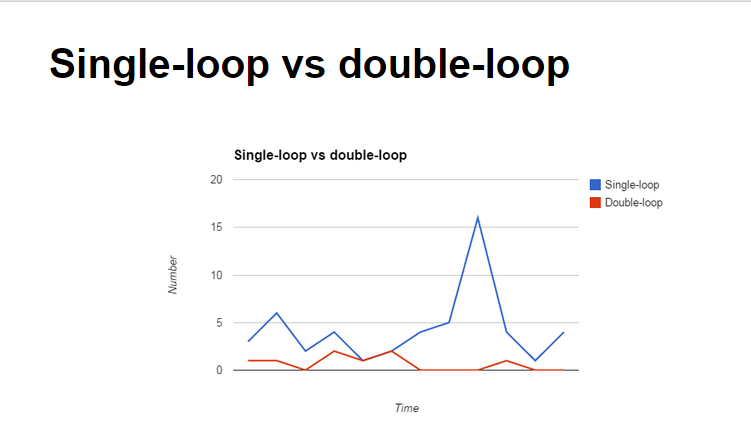
\includegraphics[width=\textwidth]{figures/Pilot_loop.PNG}
	\caption{An example of a slide from the pilot study presentation }
	\label{figure:Pilot Slide}
\end{figure}

\chapter{Content Analysis Categories}\label{appendix:categories}
The results of our pilot analysis gave us an extended set of categories that we will now describe further. Mainly we found six main themes that we could derive categories from. The six themes were: Nature, Context, Decision Making, Organizational Learning, Development and Management. We will describe each of these themes and their set of categories further in the sections below.

\section{Nature}
The nature of the action is the first theme that the content analysis is going to inspect. We define the nature of the action as how the origins of the action began. Did they come from a problem that occurred during the iteration or is it a continuation of something that has been working well in the past. Through our analysis we will try to understand the origins of the actions and classify them either as positive, negative or undefined. We define our classifications below. 
\paragraph{Positive} Positive actions is those actions where the origins of the action is in a positive context. If the action represents a current good working practice being continued, or something uncommon happened that gave positive results, it would be classified as positive.
\paragraph{Negative} The negative actions are those actions that has its origins from a problem or abnormal issue resulting in negative results. If an action is a result of a problem or abnormal issue it is classified as an negative action. 
\paragraph{Undefined} In the cases where it is unclear whether the origins of the action is positive or negative we classify the action as undefined. Such occurrences can be a result of missing context or actions that seem to have neither positive issues or negative issues as its origin. 

\section{Context}\label{method:context}
The context surrounding the action will be analyzed. The context off the action is based on the underlying issue that leads to the needed action. We divide the issues into three main categories, technical, process and undefined. 
\paragraph{Technical}
A technical issue can be a issue relating to technical competence, bugs or problems.
\paragraph{Process}
A process issue stems from a problem with a process, or potential for improvements in the existing processes. This can for example relate to communication between colleagues or work scheduling.
\paragraph{Undefined}
 An undefined issue might not have any clear origin, or might be too loosely described to be classified easily.

\section{Decision Making}
Rational decision making is how decision makers should think and should act based on coherence and rationality, according to M. Drury et al. ~\cite{Drury2012}. N.B. Moe et al. ~\cite{Moe2011} appends bounded rational decision-making as the means of understanding how decision making is made in non-routine activities. N.B. Moe et al. reasons that both are needed when analyzing decision-making in an agile context:
\begin{quote}
Software development involves both routine and non-routine activities. Hence, it makes sense to use both rational and bounded rational decision making theories when explaining decisions in software development processes. 
\end{quote}
Drury et al. distinguishes between two types of decisions being made in an organization, the strategic and the tactical. Moe et al. distinguishes between three types: Strategic, tactical and operational. We will use the three-type model. Each decision type will be described in the following paragraphs. 
\paragraph{Strategic}
A strategic decision is a wide ranging decision dealing with multiple or sizable issues, often causing major changes and have a long term impact.Moe et al. describes the strategic decisions as the following: 
\begin{quote}
Strategic decisions are related to organizational goals and objectives. The information concerning such decisions is usually incomplete and the decision-making process may extend over a considerable period of time.
\end{quote}
The actions that are categorized as strategical is the ones that proposes changes that have a long term impact or proposes changes that are related to the organizational goals. 
\paragraph{Tactical}
A tactical decision is smaller than a strategic decision it seeks to deal with the distribution and use of resources available to the team. Moe et al. described it as: 
\begin{quote}
Tactical decisions are related to identification and use of resources.
\end{quote}
All actions that specifically proposes to identification of resources or proposes changes to how resources are spent will be classified as tactical.
\paragraph{Operational}
Moe et al. describes an operational decision as: 
\begin{quote}
Operational decisions deal with ensuring effectiveness of day-to-day operations within the organization. 
\end{quote}
Every action that are restricted to only day-to-day operations will be classified as operational decisions. They might be quick fixes that solve a single problem. 
\paragraph{Undefined}
An undefined decision might be difficult to categorize because of a lack of context or an unclear description.

\section{Organizational Learning}
Organizational learning is a process where an organization takes steps to improve its current work environments by reacting to issues that arise. These steps can be varied, and we divide them into single-loop, double-loop and undefined. Retrospectives have a central role in 	organizational learning, as described by Dingsøyr ~\cite{Dingsoyr2007}
\paragraph{Single-loop}
A single-loop action is an action designed to change or tune a process in order to improve it. The action does not seek to address underlying problems, and are a single-feedback loop from observing an issue to making a change. A retrospective can facilitate single-loop learning where the project team uses the input during the retrospective to make adjustments to their current work ~\cite{Dingsoyr2004}
\paragraph{Double-loop}
A double-loop action is designed to solve an issue, as well as address the underlying cause of the issue. This requires an understanding of the underlying issue and the nature of its influence. Double-loop decisions can be facilitated through a retrospective, often these are as a result of a more drastic need for change and an understanding of the underlying problem. ~\cite{Dingsoyr2004}
\paragraph{Undefined}
An action might not be clearly described, or the nature of the action can not be interpreted. We will classify these actions as undefined.

\section{Development}
An issue that is related to the development of the product is included in this category. The development process is the actual work performed to create the product, as well as processes directly related to this work. The different categories included in development were chosen after discussing with advisors, as well as personal experience from the writers
\paragraph{Development}
Development includes the writing of code, specifying requirements, construction the system architecture and other aspects of designing of the system. 
\paragraph{Planning}
An action that is categorized as planning is when the action is suggesting changes to planning in future iterations or is a result of an issue occurring in a former iteration. Estimations, task-prioritization, scheduling and etc. all goes under the planning category.
\paragraph{Testing}
Issues related to the testing of a product, this includes unit, module and system testing. Issues related to testing can also be communication between testers and developers.
\paragraph{Documentation}
Action that are categorized as documentation is those that are related to the documentation part of developing a system. Typical actions are those that describe or propose changes to documentation practices. This can also include tutorials that explains the product and improves usability. 
\paragraph{Builds}
During development of a software system building the software system can be a tiresome task. The actions that are categorized as builds are those who proposes practices that changes the current build practices.
\paragraph{Release}
When a system feature or a part of a system is finished, usually at the end of an iteration, one deploy the new part of the system into production, available for the users. For the actions that categorized as release, the action describe some aspect of the release practice and either proposes changes or suggest new practices.
\paragraph{Business}
Business development is a critical part for an organization to create profit. Software system often can save costs and create new business opportunities and as a part of a software development team one also has to consider business perspectives. We categorize all actions that are related to business development or proposes some business related changes as business. 
\paragraph{Undefined} If an action is neither of the development phases described above we classify it as undefined. 

\section{Collaboration}
One of the aspects during a software developing process is collaboration. Fægri ~\cite{Faegri2012} describes collaboration as the following: 
\begin{quote}
Collaboration is a key aspect of software development. Collaboration allows groups of software practitioners to deal with uncertainty, complexity and interdependence. And in dealing with these challenges, the group demonstrates its collective problem-solving ability.
\end{quote}
Through our pilot analysis we registered several activities that are related to collaboration. Communication, leadership, competence, external relations and planning all belongs beneath the collaboration banner, and we describe in detail how we classify each of them below. 
\paragraph{Communication}
Communication is a widely used word and concept, but it rarely is defined. By using Merriam-Webster dictionary ~\cite{MerriamWebster2015} we found a definition that can serve as a clarification: 
\begin{quote}
The act or process of using words, sounds, signs, or behaviors to express or exchange information or to express your ideas, thoughts, feelings, etc., to someone else.
\end{quote}
Nakakoji et al. ~\cite{Nakakoji2010} distinguishes between two types of communication related to software development, coordination communication and expertise communication. The first one being the process of coordinating the development activities and the last one being when a developer obtain some information regarding a software artifact, either through code comments, wikis or other means. 
We are however not going to distinguish between these two communication types in our content analysis as we believe the two differentiations is covered by the context of the action as described in \autoref{method:context}. For our content analysis we are simply going to count every instance of communication for every action that is related to communication between team-members regardless if it is through text, speech or other means of communication.
\paragraph{Leadership}
As is the case with communication, leadership is also widely used concept, that is rarely specified. Again we turn to Merriam-Webster \cite{MerriamWebster2015} for a definition: 
\begin{quote}
The power or ability to lead other people.
\end{quote}
Agile development teams is often self-organized as it is one of the principles in the agile manifesto \cite{AgileManifesto2015}. This can result in no clear leadership. For our content analysis we are going to consider decisions and guidelines set by the group itself as leadership activities. We categorize actions as leadership if they somehow suggests changes to leadership or if the actions is a result of some leadership related issue. 
\paragraph{Competence}
We define competence as the ability to perform a certain task in a adequate quality. Each member within an agile team has their own set of knowledge that they use to solve different tasks. If any issues arises and the group is lacking the knowledge to counter it we categorize the action created to resolve it as an competence action. An example could be issue of lacking the knowledge resolving a database error and the action is to send one developer at a database course. This action would then be categorized as an competence action.
\paragraph{External Relations}
By the category external relations we mean if the team has any actions that is a result of issues arising from external factors or the actions that team is creating to inflict some external factors. Example of external relations can be customer relations, communication with server maintenance team or other development teams.   
\paragraph{Undefined}
For those actions that the origin is unclear and the goal is not related to any of the collaboration categories we categorize them as undefined.

\chapter{Shared Mental Models}
\label{section:mental-models}
The theory of shared mental models is from cognitive psychology, and can be used as a lens to evaluate agile development and methodology as described by Petter et al\cite{Petter2013}. The concept is that a team has a shared mental model that is central to the mutual understanding between team members, and thus essential to project success. Without a good shared mental model a team is left with a poor understanding of the task at hand, as well as barriers for cooperation. Two metrics used to measure a team's shared mental model are ``similarity'' and ``accuracy''. Where ``similarity'' is the degree which the shared mental model is similar between team members, and ``accuracy'' is the degree which the shared mental model matches objective measures. 

\section{The stages of Shared Mental Model generating}

\label{section:mental-models-stages}
	
Four different stages of building shared mental models are identified \cite{Petter2013}. These are knowing, learning, understanding and executing. An overview of these stages is seen in  \autoref{table:stages-mental-model}. Knowing is the stage where a team gets exposed to information relating to their project and project goals, at this stage team members are encouraged to share information between each other. The second stage is the learning stage, this stage consists processing the information gained in the knowing stage. The understanding stage is defined by reaching consensus and understanding the team member's individual views. Executing is the last stage, with a developed shared understanding the team is able to reach goal, at this stage a team responds to a situation based on the work done in the previous stages.

\begin{table}[!h]
	\begin{centering}
	\caption{Four stages of mental model building}
	\label{table:stages-mental-model}
	\begin{tabular}{l | p{0.7\textwidth}}

	\hline
	Stage & Description \\
	\hline
	Knowing &  Information exposure and sharing\\
	Learning & Information processing \\
	Understanding & Consensus and common ground \\
	Executing & Shared understanding and  \\
	\hline
	
\end{tabular}
\end{centering}
\end{table}

	
\section{Shared Mental Models and retrospectives}

Petter et. al. \cite{Petter2013} describe multiple agile development practices, but do not focus a lot on the agile retrospective. In the appendix of the article they give the following link between retrospectives and shared mental models.

\begin{quote}
Enhances the development of learning and understanding stages by facilitating the information sharing and integration. This practice also improves the teams’ executing capability in the next sprint
\end{quote}

The shared mental model practices that are involved in the retrospective are identified as self corrective, training and reflectivity. We discuss the relationship between our results, retrospectives and shared mental models in \autoref{section:shared-mental-models-discussion}.

\chapter{Transcription: Interview SCRUM Master - Team Zulu}
Researcher 1: Vi er interessert i hva du tenker som scrum master først og fremst. Hvordan du opplever ting, samt elementer fra presentasjonen også om det var noe som overrasket eller noe du savna.

SCRUM master: Ja altså det var jo interessant, vi jobber med dette hele tiden. Vi har ett veldig sterkt forhold og eierskap, men vi har aldri gjort dypdyk eller kategorisert de forskjellige ... tiltakene. Så det var veldig interessant å se  at liksom trendene, det er ting når man liksom har en følelse av hvordan det ser ut, men det er en annen ting å se det i en graf. Jeg hadde visste ikke helt hva jeg skulle forvente, jeg visste jo litt siden jeg hadde snakket med dere, så jeg visste nok mer enn de andre, men jeg synes det var veldig bra, veldig interessant.

Researcher 2: Glimrende, nevnte det om trender da, og det er jo noe vi er redde for å uttale oss om, vi skjønner jo at dette bare er en liten del av bildet. Men i forhold til hvordan vi forklarte vår tankegang, gi det mening når du så det i det store bildet da?

SCRUM master: Ja, altså dere klassifiserer så teller dere og så ser dere om det er en trend. Type sånn scenario template da så er det et virkemiddel på en måte, noe som vil dukke opp i all slags kontekst, som et virkemiddel vi bruker for å gjøre de rette tingene. Da var jeg jo overrasket om at det flata ut, men det kan jo være tilfeldig og. Det finnes mange virkemiddel for å få gjør ting, men det var jo påfallende at flere grafer flata ut tidlig på året i fjor og det sammenfalt jo da med diverse ting som har skjedd i vår avdelig, jeg har tro på at der er det en korrelasjon altså. Det er en sammenheng da, vi vet jo at dette er litt guesswork, kjenner jo ikke alt, kjenner ikke 100\% bakgrunnen til ting som dukker opp i retrospektiv, dere har jo gjort en fantastisk jobb.

Researcher 2: Nevnte jo det jo tidligere, men akuratt denne typen studie har ikke blitt gjort før så det er jo litt interessant for å se anvendelse område og hva tenker du om det som ett statistisk verktøy til analyse osv? Du nevnte om å ha det som ett dashboard?

SCRUM master: Poenget er at vi bruker jo vårt eget system, det som vi utviklier det som vi lever som produkt, det bruker vi internt for å regisstrete alle slags retrospektiver vi har, så lager vi ny sak og så lager vi actions og det har vi jo gode muligheter for å få ut statistikken. Og hvis vi hadde bare klassifisert det slik som dere gjør så kunne vi fått ut statistikken på ett dashboard, vi har andre dashboard der vi teller kommunkiasjonsfeil og trender der da, med forbedringsforslag fra kunder. Så vi kunne definitivt gjort det, det som gjør at jeg er litt skeptisk i utgangspunktet. Det som gjør meg litt skeptisk er at vi har hatt verktøy tidligere der vi har vært nødt til å fylle ut klassifisering, obligatoriske felt som man ikke kan lagre uten å fylle ut denne klassifiseringen da. Og av og til blir det litt i hu og hast litt tilfeldig valgt man har for eksemple causes, da man ikke har tid og det er grunnen til av feilen oppsto, man finner ikke den rette og kvaliteten blir dårligere, uansett så har vi ikke brukt det til noe. Vi har egentlig brukt det til arbeid til å få det riktig, men har ikke tatt ut statisitikken og brukt til noe fornuftig, og da er det waste, invistert tid som vi ikke får noe glede av. Men det jeg tror med noe tilsvarende for tiltak for retrospektiv så måtte vi passet på at vi faktisk brukte det til noe, og det er jo interessant å se, men når man måler seg selv og man har ett target og du vil nå en target og du vet at det blir målt så kan det jo påvirke det som blir sagt i retrospektiv, selv om man sikkert ikke ønsker det kan det likevell påvirke, jeg vet ikke det er litt både og. Men det hadde vært utrolig kult å få hatt litt hånda på pulsen og se hva vi gjørl

Researcher 1: Sånn som nå så har dere dette prikkesystemet, merker du noe tension på det?

SCRUM master: Ja det blir jo veldig synelig da hvis man slite litt, men det er jo hele poenget, hvis ett scenario henge på samme plassen og får prikk på prikk så er det om å gjøre ett eller annet tiltak siden det er ett eller annet problem da. Det var jo det som var ideen, nå så du jo denne ``testing'' har vært der ganske lenge, og da vet vi jo hvorfor, det var jo mye tester, over 100 requirements, da sier det jo seg selv. Men man merker det jo hos noen team members at det er litt sånn at det ligger litt synlig, men vi gjør det jo ikke for at det skal være en irritasjon men for å synliggjøre det. Da må vi gjøre tiltak, og egentlig kan det vær ett konrekt, og det er synliggjort men det er blokka. 

Researcher 2: Hvis du liksom i det ideele, har du noe du skulle ha med ressurser eller tid noen forbedringer på den eksisterende formen på å holde retrspektiver?

SCRUM master: Jeg nevnte tidligere at det er veldig enkelt sånn vi gjør det  og grunnen til det er at alle skal få en sjanse til å si noe, hvis man bare sitter løst og snakker om det så er det noen som vil gripe ordet. Og det dekker jo behovet sånn sett, men det finnes jo andre metoder for å utføre en retrospektiv. Vi hadde jo en liten demo nå på forskjellige teknikker, blant annet dette her med positive og negative ``Hva synes dere har vært positivt og hva synes dere har vært negativt?'' Hadde hele tavla full av lapper, skulle lage en sånn ``weather forecast'', det ble vi egentlig enige om at vi skulle innøre, altså ikke hver iterasjon, men ett par ganger i året. Det var interessant å se hva vi liksom fikk ut av det, men vet ikke vi har ikke egentlig ikke noe som kommer til kort i det vi har vi får frem det som, det er veldig viktig at man føler man blir tatt vare på og at man blir hørt, hvis man snakker og det er ingen som tar hensyn til det man sier, da er man dømt og man gidder ikke bidra til slutt. Føler vi har fått en kultur der alle føler de har noe de skulle ha sagt da.

Researcher 2: Det vi har lyst å ta noen eksempler på, at noen føler at man ikke blir tatt på alvor kan bli en negativ feedback loop der folk bidrar enda mindre og så blir enda fortere ferdig.

SCRUM master: I en travel hverdag så er det ikke alltid det passer, derfor bruker vi en time og ikke noe mer, så ofte så blir det sånn at vi kutter og tar det på neste om 3 uker, men likevell den timen i en travel hverdag kan være litt forstyrrende, men hvis vi ikke gjør det så.. vi utsetter, dropper det denne gangen så neste møte varer jo mye lenger, så folk har jo noe de vil ha sagt, så vi har konkludert med at vi måte være strenge på dette. Og har hver 3 uke. Jeg tror folk tror det er positvit. Hva spurte du om egentlig?

Researcher 2: Om du hadde noen potensielle forbedringer?

SCRUM master: Ja, nei jeg er jo egentlig fornøyd med sånn som vi har det, har ikke fått så mye input, hadde jo besøk fra sintef men det er noe vi kan gjøre nå og da i tillegg, men vil ha denne basci formen

Researcher 2: Du nevnte at noen for noen kan det være ett forstyrrende element i en travel hverdag, er det noe fokus på at det skal være en positiv opplevelse, flerne artikkel foreslår gratis lunsj eller lignende, hva slags tanker har du? Altså skape litt sånn ``festelig'' atomsfære.

SCRUM master: Det er jo egentlig ett godt poeng da, det kunne vi sikker gjort noen grep for at det skal være positivt altså, det skal jeg tenkte på. Sånn i den formen det er nå så prøver vi å ha en lett og ledig tone der vi spøker litt og ler litt det skal ikke være gravalvorlig, men noen ganger  så går diskusjonen og man har forskjellige meninger det som og gjerne kjennetegner våre diskusjoner er at vi prøver å finne consensus på en måte, og hvis man ikke blir enige så prøver vi dette og hvis ikke det går så kan man prøve noe annet senere. Men akuratt noe positiv aura rundt det... Hva har andre gjort?

Researcher 1: Noen har gratis lunsje og lignende.

Researcher 2: Noen hadde farger og stjerner til de som var flinke.

Researcher 1: Noen brukte kaker eller lignende for at man skulle forbinde det med noe positivt, det er jo mange som sliter med, mange som ikke har en positiv følelse.

SCRUM master: Ja at de ikke helt ser poenget med det. Det er noe man blir pådyttet på ett hvis, ja mitt inntrykk er at vi deler eirerskapet, og man liksom føler eierskapet.

Researcher 2: Rent akademisk, det vi snakket om med fri lunsj osv, det at man føler det positivt, hensikten er ikke bare å si at man følte dette fungerte bra, men det er også at det blir en klapp på ryggen ``bra at vi får til dette maintenance møtet". Så tenker man neste gang man skal på retrospektiv møte, ``det vi gjorde for 2 ganger siden funka" Så blir man gira for neste. Hensikten er jo  at folk skal engasjere seg så mye som mulig.

SCRUM master: Jeg ser den altså, det er ikke noe sånn organisert, typisk de som var involvert i den endringen vil gjerne si hvordan det var, og det funker kjemperbra, vi kunne nok vektlagt det mer. Sende ord videre liksom, man kan jo spør om det er noe positivt liksom,

Researcher 2: Særlig sånn her problemløsning i team, er jo veldig problemfokusert her, negativet  er kanskje litt lada ord i forhold i den sammenheng at det nødvendig er noe dumt.

SCRUM master: Det er jo negativt til man finner en løsning, da er det noe positivt igjen, når man sliter... f.eks dette med bugs og sånne generelle bugs det kan bli litt liggende og slenge. Vi hadde ett system der man skulle jobbe med det, men det ble ikke noe håndfast og man dedikerte ikke tiden til det når vi fikk den dagen, som var ett veldig enkelt grep, som har vist seg å funke veldig bra, vi ser på statistikken og at dette virker, og det blir en seier da og vi ser det er noe positivt i det. 

Researcher 2: Nå hørtes jo det ut som noe dere er veldig klar over, men hvis man skriver det ned og sier det høyt i gruppa så gir det mer trøkk.
Researcher 1: Vi gikk jo at i fjor hadde dere en(medarbeider) som gjorde at ting ikke helt funka og at retrospektivet ble litt sån taust, og det har vi egentlig fått høre nok om, men har du noen andre tilfeller hvor enkeltpersoner kan være destruktive for retrospektivet?

SCRUM master: Ja jeg skjønner hva du mener det er jo generelt i team da, i agile der man ønsker liksom at teamet skal ha noe de skulle sagt så, sånn at man føler at man bidrar, da er det jo noen som kan ta helt over. Det er ett moment, men det har jo gått bra, det er jo noen i teamet som har mer de skulle ha sagt enn andre. Men tror vi har funnet en vei. Bekymringen er jo, sånn generelt, at man skal bli arrestert hvis man kommer med noe, men det er såpass mye respekt mellom teammedelemene at det går greit, det som var saken, med han som slutta var jo det at han forårsaka så mye misforståelser og problemer at det overskua alle andre problemer. Det var i grunnen elefanten i rommet, det er jo klart alle nyansettelser eller folk som slutter eller hva det skal være alle forandringer i gruppa vil jo forandre dynamikken, da må man liksom finne en ny måte å inrette seg på. Det er jo et interessant spørsmål. Det er vell det beste eksempelet jeg kan huske.

Researcher 1: Er det noen som er veldig stille?

SCRUM master: Det er det, helt klart. Og de komme jo med sine ting de og, men det er bare det at har ikke behov for å markere seg i rommet når de får ordet så har de jo kanskje ting som de har tenkt på. Jeg har jo tenkt på det. At de ikke skal være helt for sakte. Det er jo en ting som ikke nødvendigvis ikkke skriker ut, men jeg føler jo at de bidrar

Researcher 1: Føles ikke det destruktivt eller hindrer ikke fremgang?

SCRUM master: Nei, eller jeg vet jo ikke dette 100\%, jeg går ikke til de og annonsere.. de sa ingenting de som ikke bidro, så måtte jeg vite hva det var.

Researcher 2: Men det er liksom innenfor rammene så er det greit.

SCRUM master: Ja folk er jo forskjellige.

Researcher 2: Det er ett par vi snakket med under lunsj, med han dere hadde problemer med så nevnte de en del sånn der kulturelle forskjeller som førte til problemer da. Har du noen mulighet til å uttale deg om det?
SCRUM master: Ja det har jeg, det er jo åpent. Jeg tror alle i teamet er klar over det, vi har jo snakket om det og, vi har jo.. noen kulturer ønsker å ha alt skriftelig med fem signaturer liksom, og et må inn med teskje. Det er ikke sånn vi jobber,det er ikke sånn vi jobber, vi speccer det er ganske sånn lauslig (løst) Får en handover fra arkiteteken går jo gjennom det så får vi en forståelse og tar litt underveis og da er det jo selvfølgelig en periode i begynnelsen før de blir vant me dette føler jo at de drive jo litt med god arbeidskultur og god skikk. En annen ting er jo tap av ansikt hvis ikke man forstår noe, og det er vi jo helt avhengig av. ``Forstår du ikke hva jeg sier til deg?" ``Ja jeg gjør jo det" og så er det åpenbart etterhvert at det var ikke forstått, man forsto ikke. Trenget du hjelp? og så trenger man ikke hjelp. det fungerer jo godt i Norge da. Det er jo litt det å være off da.

Researcher 2: Nevnte jo det at man ikke hadde lyst å være frekke foran denne personen under retrospektivene da.

SCRUM master: Ja det blir jo veldig personlig, det er jo det som er liskom. Det går liksom på personlighetstrekk og på... Retrospektiv er ikke skapt for denne type ting, det må håndteres på ett annet nivå.

Researcher 2: Det som gjør det for oss er jo det at en personalsak kan påvirke enn annen prosess, det er jo det som gjør det interessant for oss.

SCRUM master: helt klart.

Researcher 2: Nå skal jeg ikke legge ord i munnen din, men si dette problemet med medarbeideren da, tror du at det fantes ganger der de ikke gadd å ta opp andre ting heller, siden de tenker, vi får uansett ikke løst det store problemene, så kunne vi kanskje tatt dette og.

SCRUM master: Det er sånn! Det overskygger. Det er litt sånn,

Researcher 1: Store problemer overskygger de små?

SCRUM master: Ja det er generelle ting. Da blir all fokus på det problemet de mindre trivielle problemene dukker ikke opp før man har løst de andre. Nå var jeg i permisjon når det storma som verst, så har likom blitt fortalt hvordan det var. Det var jo... En ting var at det ikke funket å godt under retrospektivet, men det tærte jo på teamspiriten generelt. Det er jo nok bare ett symptom på ett underliggende problem at retrospektivene ikke funker. Men det er jo klart, det så ble gjort i kulissene er jo at den som fikk personalansvar fikk jo beskjed om alle problemene, og det var opp til ha å gjøre tiltakene, men det er jo ikke så veldig enkelt. Man vil jo helst få det til å fungere.

Researcher 1: Hvordan, store problemer, hvordan takler dere det, hvis de kommer opp på retrospektiv, hva gjør dere da? Setter av tid eller?

SCRUM master: Ja, det kan vi gjør, men for meg dukker de opp før retrospektiv. Hvis det er veldig.. så tar man jo tak i det der og da. Det som vi og kan se er jo for eksempel at vi hadde ett scenario der vi hadde problemer, der det var litt kommunikasjon, og det var litt diverse sånn der, mellom testere og utvikler, nå har vi laget ett retrospektiv kun for de som var involvert og så skal vi sette og ned og finne ut av det. Det blir litt ad hoc. Tenkte jo at vi skulle ta det opp som ett vanlig retrospektiv. Men det er bedre at vi bare tar det det gjelder og så heller deler vi det vi finner og deler med alle.

Researcher 1: Hva skal til for at noe blir tatt opp? Må det vært snakka om før?

SCRUM master: Nei, det er ikke sånn. Noen er veldig flinke og noterer underveis og lager seg en liste om ting de vil snakke om. Mens andre er litt sånn hva var det jeg gjorde siste uke og må tenke etter liksom. Det er sikker og personlighetsforskjell da, noen er veldig metodiske og andre er mer ad hoc, på sparket. Men det er jo... egentlig så har vi, vi ønsker å fokusere på prorsess, det er jo det som egentlig er hovedfokuset, men vi har ingen grenser for hva vi kan snakke om, det blir  litt sånn klassisk team.

Researcher 1: Ja forsåvidt, føler du at teamet er ærlige eller trygge på hverandre gjør du noe for å fasilitere trygghet? 

SCRUM master: Ja altså, jeg føler at de er trygge på hverandre, de fleste har jobbet lenge sammen, men det er. Jeg ser. Et annet eksempel på at kjemien ikke har vært så god da, det var en som for stund siden, det var alltid en greie mellom han og testeren da, det ble liksom personlig fant man en bug så ble det. Åh nå fikk jeg en bug på meg igjen liksom. Følte at han måtte forsvare seg på en måte, og da ble det mye gnikkinger på det mellom testeren og han der utvikleren da. Men da blir det liksom en personssak. og det er sånn som ikke dukker opp i type retrospektiv, men det blir mer sånn som kommer frem gjennom linjene, man snakker i generelle ordlag mens egentlig så snakker de om hverandre.

Researcher 2: Det blir lit sånn passivt aggressivt. 

SCRUM master: Ja, og det er ikke bra, men det er jaa, jeg føler at de aller fleste er ganske åpne med hverandre og snakker direkte med hverandre om det er noe som ikke funker, derfor er det og... altså eneste er kanskje hvis du kommer for en annen kultur der du føler at du ikke skal motsi de du oppfatter som ledere på en måte, så blir du usikker på om de er enige eller om de bare later som.

Researcher 2: Det finnes litratur som sier at et retrospektiv ikke bør ha med ledere folk som har autoritet da.

SCRUM master: Ja, men vi er jo Norge da , og vi er veldig flate i utgangspunktet nordmenn har ikke respekt for lederene sine, det er jo den store fordelen, med å ha de med er jo at når man gjør beslutninger er jo at, Jan Edvard, da kan man jo ta større avgjørelser og trenger ikke sjekke med ham først da. Det er litt positivt og negativt. Men den littraturen jeg vet ikke hvor de kom fra de som har skrevet den, men det er typisk i hierarkiske kulturer da. Da vil jo lederen være veldig negativ å ha, men vi har jo folk fra andre kulturer da, og da dukker jo dette opp etter at de har aklmiatisert seg og... det må jo vær ganske forvirrende tenker jeg. 

Researcher 1: Opplever du at du blir sett på som en leder når du leder retrospektiv eller mer enn fasilitator?

SCRUM master: Ja mer en fasilitator ja, men til dagelig at de kommer til meg, altså de kommer til meg med prosessforslag eller ting som de vil ta opp på retrospektivet da. Det er jo ikke for at jeg er leder, men fordi det er jeg som organiserer det. Men føler meg ikke som leder av team. 
Jeg får jo litt mer ansvar på ett vis, det er... selv om jeg er en del av teamet når jeg fasiliterer så må jeg egentlig ikkke... det er ikke sånn at jeg motsier dem, hvis de kommer med noe og det er en dårlig ide. Det er mer at jeg søker consensus og så ``synes alle det er en god ide?" liksom. Men vi kan jo kanskje i den rollen.... jeg er jo veldig observant på hvordan ting flyter. Så noen ganger kan jeg komme med radikale ting da som jeg... som jeg har lest om og som fungerer, men jeg tror ikke de ser på meg som noe leder.

Researcher 1: Blir det godt mottatt, radkale forslag? Eller? Eller er de ofte skeptisk?

SCRUM master: Det er rart... Vi holdt på ganske lenge med retrospektiv som vi har holdt på med kontinuerlig forbedring ganske lenge ikke sant? Det er ganske lett å komme med bra ideer, så kan det være at jeg blir klubba ned og det var ett dårlig forslag ikke sant men ofte er det sånn at ja vi kan prøve det og så prøver vi det en iterasjon og så ser vi hvordan det går. Det med de ``lanesene" da det var jo noe om Kirsti kom med, hun hadde vært gjennom en periode i statoil og der gjorde de det. Så prøvde vi det og sånn ble det.

Researcher 2: Fornøyd med det?

SCRUM master: Ja vi har vært fornøyde, jeg tror generelt sett at folk er fornøyd med det, jeg har.. jeg driver egen tenking det flyte ikke helt 100\%. Kommer til å foreslå noe snart.

Researcher 1: Når dere kommer opp med de tiltakane, noen ting er jo ting dere har nå, men hvor henter dere andre ting fra? hvis dere kommer med noe helt nytt som ikke har vært noe problem, er det noe dere har lest? Eller diskutert rrundt lunsjbordet?

SCRUM master: Hvis det er noe som ikke funker så er det ofte at vi har 2 eller 3 stykker som kommer opp på en eller annen måte og så ser vi på, blir det litt sånn at man får en teori om at hvis vi hadde gjort sånn og sånn så hadde det fungert, og da dukker det opp på retrospektiv. Da er det jo masse er selvsagt men og hvis vi har vært på konferanser eller kurs eller ett eller annet sånn og vi har fått noe inspirasjon fra det, eller.. vi jobber jo tett med andre team og man får noen innspill derfra som dukker liksom opp, og så skal man prøvd det likosm. Vi er jo ikke sånn at ... inspirasjonen her.. Vi begynte jo med SCRUM, men nå er vi ganske langt fra scrum, og det har vært en kontinuerlig prosess da, for å forbedre og få ting til å funke bra. Så har vi jo endt opp.... Nå er vi jo nærmere Kanban enn SCRUM, men det er jo klart man blir inspirert altså, når man går på MVC og hører om metodikk og lean og alt det der. 

Researcher 2: Rent i fra vår oppgave, så tenker vi på retrospektiv og særlig da organisatorisk læring ikke bare innad i teamet, at det skal smitte på en måte. Og det er da det med positive tiltak så folk på utsiden skal se hvordan forskjellige action oppleves. Har du noen tanker rundt det?

SCRUM master: Hva betyr det? positive tiltak.

Researcher 2: Si nå for eksempel denne bug dagen, hvis noen da skulle lest gjennom det senere, som dokumentasjon eller lignende så er det ikke nødvendigvis at de hadde skjønt hvor positivt det oppleves for dere.

SCRUM master: Ja det nevnte vi jo tidligere og, ja men hvordan skal du... altså... De tiltakene vi lager de er jo noe man skal gjøre, det som funker det endres jo kanskje ikke, dont change a winning team. Men tenker du at det skal være dokumentert, burde da være synlig på en måte? Notable efforts på en måte? Ja! Det kunne vi faktisk ha gjort, at man på en måte registrerte det. At det ble ett moment på en måte, det som ble nevnt som var positivt det la jeg inn i noe. 

Researcher 1: Sånn sett, hvis det er noe du skal legge inn i fremtida kan jeg si nå har jeg lest gjennom actions så er det mye som, hvor konteksten blir vanskelig så hvis du skal sende til... så er det kanskje verdt å fortelle... hva som er grunnproblemet. 

SCRUM master: Ikke bare det du skal gjør liksom? Vi har gjort det mange ganger da, pga sånn og sånn så må vi gjøre sånn og sånn, det tar jo tid og, og etter noen møter så sitter man igjen med sånn 10 tiltak og så tar det helt av liksom. Men ja, jeg ser den, det er jo ikke så mye arbeid å gjøre det, notable efforts ja. 

Researcher 1: Nå har du fortalt hvordan dere holder retrospektivene, men har det endra seg underveis? Gjort det på andre måter?

SCRUM master: Nei vi har egentlig fulgt den samme tråden, men jeg føler at det har blitt mer ett delt eierskap til det nå da, enn det var tidligere da. Man ser sammenhengen liksom. Man utfører tiltakene man kommer frem til da.

Researcher 1: Er det noe som har kommet i senere tid nå eller er det noe som har kommet...?

SCRUM master: Gradvis, det er en modningsprosses da, når vi begynte med SCRUM, eller Agile i det hele tatt, så var jo det sånn naturlig skepsis, det var ikke alle som bare omfavnet det liksom.

Researcher 1: Når var det dere gjorde det liksom?

SCRUM master: La oss si... midte på 2000 tallet. 2004-2005 liksom?

Researcher 2: I den perioden?

SCRUM master: Ja da begynte vi liksom å ha litt stand up, da sto vi bare i en ring og snakka om det, men da va ideealet scrum, men det fikk vi ikke helt til å fungere. Min personlige oppfatning er at SCRUM er litt det som ikke funka har forfalt, man planla en sprint og skulle gjøre de tingene, men så endte man opp med å ikke komme i mål, da har man på en møte brukt masse tid på å estimere hvor mange timer man skulle bruke for at man skulle gjøre det innen disse ukene liksom. Så skled det over i neste sprint også ble det bare sånn alt forskjøvet. Jeg har egentlig mange grunner til at det ikke fungerte.

Researcher 2: Det er jo veldig interessant uansett

Researcher 1: Det blir litt SCRUM but something else.

SCRUM master: JA, jeg tror det er en bra ting, jeg tror det er viktig at teamet på en måte finner sin vei. 

Researcher 1: Nå vet jeg jo ikke hvordan actions gjøres i sånnsett, dere tilgegner en person til å gjøre en action, er det noen spesiell grunn til at en person blir utvalgt eller er det bare en formalitet?  Som får ansvaret for den utførelsen.

SCRUM master: Ja det er en annen, vi driver litt sånn push egentlig. Men nå er det litt sånn krefter i teamet da som heller mer mot pull og i ett pull så blir det ikke assigna men det ville lagt der. Men som sagt akuratt nå er det mer push basert og da er det sånn han er god på det og han er det og sånn, det er bare det.  Så er det litt sånn at hvis du ikke får det så gjør man det ikke, man har ikke basert noe pull system. Hva tenker du om det?

Researcher 1: For vår del har vi som konklusjon at det man ikke kan se hvordan man holder retrospektivet, men gjerne oppfølgningsbiten etterpå er det man sliter med, det kan demoralisere og gi en negativ feedback. Spørsmålet er at for dere som er ett team som det funker veldig bra så er vi interessert i hvordan dere gjør det, hvordan dere gjør den oppfølgingen etterpå.

SCRUM master: De tiltakene som blir gjort  med en gang,og ofte er det jeg som gjør dem, type de med scenario template, så jeg gjør det med en gang, men de større overgis til noen andre som må gjøres, hvis det er noe bygging så kan ikke jeg gjøre det. Og det assignes som en task, og da blir det Ross for eksempel som må gjøre det.

Researcher 1: Gjelder det alle tekniske ting at det liksom blir assigna?

SCRUM master: Vi har jo litt forskjelllige kompetanse så det kommer ann på hva vi får, men vi har.. vi sliter litt, vi har ikke helt funnet formen på liksom vi skal... det er ting som på en måte har ligget litt som vi egentlig burde fått igjennom, men  det kan vær at vi innkluderer det i maintenance dagen, og liksom gjør det til en greie da. Da kan vi gjerne henge lapper på det som er av tiltak..

Researcher 1: Hva med sånne prosessendringer som krever litt mer effort? Er det noe som man tar seg tida til å innfører underveis eller er tas av scrum master eller?

SCRUM master: Det er ett problem faktisk, folk blir enige om å gjøre det sånn men man har ikke noen måte å enforce det på, vi har ikke... så sklir det alltid litt ut, vi har ett dokument, som heter development policy, som der er på en måte ting vi har blitt enige om at sånn og sånn må vi gjør det. Det legger vi inn der. Det er på en måte det vi har da. OFte er det sånn at man må huske det selv. Også bruker vi type. For eksempel code review, det gjorde vi ikke for noen år tilbake siden så hadde vi ikke code review. Nå må man via code review før det passerer videre ikke sant. Man trenger enn eller annen måte å enforce det på. Det er ikke alltid like lett men vi prøver å finne en måte som liksom gjør at dette vil bli gjort. Et annet eksempel er jodet med disse lansene ikke sant, der var det jo en ganske stor endring. Og det var det jo jeg som tok ansvar for, 

Researcher 2: Det var veldig linje.

SCRUM master: Jaja, sleit lenge med dem. Det er faktisk sånn tape ment for whiteboard, tips hvis dere noengang skal gjøre det, får kjøpt de. Ja. Da slipper du å bruke spirttusj, hvis du noe skal endre på noe senere så slipper du å kjøpe nye whiteboard. 

Researcher 1: Ja du skulle sett vår på kontoret, det er skjeve linjer.

Researcher 2: Litt alternativt.

Researcher 1: Hva med sånn, ren spekulasjon hvis vi har jobbet i en bedrift i syv år, det som du har,... empower... selvinnsikt, det vi har gjort er hengt opp en tavle, på rommet, hvor dette er fokuset, og har linjer så du hele tiden ser hvor man er, ute på lunsj eller. Har du vurdert å innføre noe sånnt noe? Visualisere, synliggjøre noe sånt noe? Tiltak som dere har satt som fokus for eksemepel et fokustiltak litt tidligere da.

SCRUM master: Nei! Det er jo en måte å gjøre på, den policyen vi har.. det er jo mange små ting og tang som skal gjøres de som har gjort det får det inn i ryggmargen, men jeg er sikker på at hvis jeg går igjennom den policyen nå så kan jeg plukka ut ting som ikke er aktuelt lenger, som vi ikke gjør lenger. Det er jo litt av det som er grunnen til at vi har møtene som skal gå i gjennom utviklingsprosessen.Det ene var scenario templaten. Vi har jo transkibten, og da ser vi er dette håpbløst er det noe vi kan fjerne her, det er jo en god del der. 

Researcher 1: For oss er det litt sånn tid, ti bud aktig. Hvordan vi oppfører oss, ting vi gjør, hvordan med teamet osv.

SCRUM master: Høres veldig bra ut hadde dere retrospektiv og da eller?

Researcher 1: Nei jaaa, det er noe vi ofte har hatt stående, det er bare noe remindere vi har for oss sjøl, om det bare er en post it lapp på kjøleskapet, kjøpe melk liksom, sånt noe da eller den typen. Vi prøvde eller jeg prøvde å innføre litt sånn agile tankegang der hver selger skulle sette sitt eget mål på en postit lapp og nå det målet var oppnådd så kunne de sett det på andre siden av tavla og det funka ganske bra den måneden vi kjørte det men det ble for dårlig enforca når vi hadde gjort det en måned.

SCRUM master: Alle på en måte.. må vær committa på en måta

Researcher 1: Nei det var ikke så lett.

SCRUM master: Som regel så er det ganske motstand mot endring egentlig, men det er naturlig refleks, man ønsker ikke endring 

Researcher 1: Er det stor motstand mot endring her eller?. 

SCRUM master: Nei altså, det er det jeg nevnte, det er slutt i teamet, man på en måte omfavner endring, ja det var en god ide det gjør vi. Det er bedre det enn andre veien, jeg har oppfatta at det har litt med at man har holdt på lenge og at man får litt sånn kultur for det da. Man kan faktisk se at det kan fungere å gjøre ting anderledes, men en god motivasjon for endring er jo at du har ett problem. hva slags butikk var dette?

Researcher 1: Jobbet i dressmann i 7 år, vi kjørte det konseptet i februar og da bli vi månedens butikk. Så det funka jævla bra, men sjefen var litt dårlig å enforce fra den lykkerusen av å vinne månedens butikk.

SCRUM master: Hvilte på laubærene, men det har jeg tenkt litt på man blir veldig fast..

Researcher 1: Greit med sånn post it greie.. man kan være frustrert over hvordan man arbeider.

SCRUM master: Men det kan jo lett bli overført til andre industrier. Kanban det kommer jo fra... den lean tankegangen... er jo fra Toyota det kommer jo ikke fra software. Flere spørsmål?

Researcher 2: Tror vi er på slutten

Researcher 1: Hva med dette?

Researcher 2: Det er jo egentlig tatt

SCRUM master: Dere kan jo bare sende en mail og!

Researcher 1: Ja vi kan sende hvis vi kommer på noe.

Researcher 2: Den?

Researcher 1: Ja! Eksterne fasiltatorer er ofte anbefalt når man holder retrospektiver for da får man ett objektivt øye på det på en måte? Er det noe dere har vurdert å gjøre eller hørt om for den saks skyld? 

SCRUM master: Nei!

Researcher 2: Dere hadde jo besøk av Nils (Brede Moe) i...

SCRUM master: Ja! Det var jo ett eksempel på det da, da holdt jo han retrospektiv for oss og da gjorde vi det på ett litt annet måte da. Det var jo veldig positivt det, og det kom jo fram en del, blant annet denne bug crush dagen, det var egentlig noe vi fant ut da. Det funka jo greit da. I praktisk må man da... er det noe, en annen organisasjon?

Researcher 1: Nei, vi snakket med NIls om det i sted også, og det er noen bruker de i samme bygget, sånn sett, veldig få som leier inn sånn sett, men finner andre personer som kan holde, som ikke har noe forhold til porsjektet sånn sett. Annet ett han kommer og kjører ett retrospektiv en gang i blant.

Researcher 2: Det kan ikke bare gi ett objektivt øye men folk blir da... de normene som ofte eksisterer i ett team, om at man kan motsi lederen, det blir liksom at man må forklare det til denne personen som ikke kan det, ``grunnen til at vi gjør det sånn er at....?"

SCRUM master: hehe, ja hva var det nå igjen. Ja jeg forstår den. Ja vi har jo ett annet team, disse konsulentene, men de driver jo ikke med scrum da, men vi kunne jo kanskje fått til noe, de burde jo kanskje...

Researcher 1: Eller tror du gruppa ville gitt motstand og beskytta gruppa? Kan det være tilfelle at noen blir redd for å tape ansikt for eksterne fasilitatorer.

SCRUM master: Det kan jo det, men det var ikke mitt inntrykk at det var sånn når Nils var her, jeg tenkte kanskje at man ville ikke bidra så mye kanskje. At man kanskje. Nei det var ikke sånn. Jeg tror nok det kunne vært tæft. Men da vil denne fasilitatoren ta del i diskusjonen og være aktivt med. 

Researcher 1: Foreløpig er vi gått grundig innen problemet på en måte som er innenforståt, men på en måte ikke fulstendig forstått.

SCRUM master: Er det sånn at det er sånn hver gang eller bare en gang iblant?

Researcher 1: Det er det vell ikke sagt noe særlig om sånn sett.

Researcher 2: Jeg mener den ene Torgeir artikelen så var det release retrospektiv, eller de større retrospektivene...

Researcher 1: Ja jeg tror kansskje det var noe sånt noe.

Researcher 2: Det var sjeldent at det var hver eneste gang, men å ha liksom ett innslag anbfeles i flere verk.
SCRUM master: Det er joe noe vi sikkert kunne... måtte bare funnet noen som kunne gjort det, kanskje funnet noen på konsulent avdelingen kunne ha... De er jo ikke helt fremmed.. De har jo bare gått av å vite mer

Researcher 2: Da blir det organisatorisk læring.

SCRUM master: Vi har jo demo møter da, da inviterer vi rubbel og bit support vi snakker jo med de, og så har vi konsulentene de inviterer vi med, hvis de får fakturere oss. De liker inntjening. Men kanskje en av de lederene der kunne, hvis vi får med de. Hva slags bøker har dere lest?

Researcher 1: For de meste forskningsartikler sånn sett, er det vi har fokusert mest på, forprosjektet vi hadde i høst var det vell 14 artikler som vi brukte.

SCRUM master: På NTNU?

Researcher 1: Fra hele verden. Mye av den forskningen er vell egentlig gjort i utlandet, finland er gjort en del.
Researcher 2: Visstnok ett team i finland som er helt rå på det der med retrospektiv, så det er en greie:

Researcher 1: Ja så vi har jo det, forprosjektet vårt gikk på å gå igjennom alle disse artiklene og se på forskjellige teknikker og sånt noe da. Vi kan jo sende deg den hvis du vil. Så kan du se den med referanselista.

SCRUM master: De er offentlige tilgjengelige?

Researcher 1: De er vell egentlig ikke det, noen er det, noen må du kanskje ha tilgang til en forskningsdatabase, web of science eller noe sånn. Journalene er henta fra der og IEEE.

Researcher 2: Vi får jo da studenttilgang.

SCRUM master: Aha.

Researcher 2: En god del av dem er jeg temmelig sikker ligger på google scholar. 

SCRUM master: Ja men hadde vært flott det, dere har jo epost adressen min.
*Resten av samtalen ble i hovedsak brukt til formaliteter*

\chapter{Team Foxtrot Email Results}
\begin{enumerate}
\item System developer - java backend / some frontend
\item The team is about 20 persons. It consists of design, ux, frontend, backend and to project leaders.
\item \begin{enumerate}
	\item Everything from every second week and sometimes not in 6 months.
	\item Retrospectives has been held in 30 minutes and up to 4 hours. Usually in less than 2 hours.
	\end{enumerate}
\item Positive aspect of retrospecives is that people gets concerns off their chest. And actions points to work with until next time.
\item No negative aspects other than all the suggested actions points are not put to life, and is repeated ``every" retrospective. Some retrospectives are too long.
\item Decisions are usually given to someone as their responsibility. Some decisions can be created as tasks in Jira. But not always followed up. 
\item If the retrospecitive is not held on a regular basis, the first retrospecive after some time will not be productive. Because it is too much to discuss.
\item The team is sort of using kanban, but in a not very strictly matter. We do not practice wip-limits. But we are developing more or less incrementally, to reduce risc when deploying new releases. It is working very good.
\item Steps to encourage learning should be more in focus. Think the answer is more or less no.
\item I'm not a scrum master. But the project lead / ``kanban" master - the person who holds the retrospectives does not seem to affect the retrospective. We have had developers (not me) leading the retrospectives with great success.
\item Retrospectives have been useful to change the way I work or think. Input from other team members is valuable. During the last retrospective I realized based on other's input that we need to communicate and make sure we are on the same page.
\item To assist decisions, experience is often used.
\item Some things can be ``solved" or agreed on straight away. Other topics require more investigation and can be followed up in the next retrospective.
\item Obstacles: long backlog and a lot to do makes it harder to take decisions, because you need to put a lot energy into it to accomlish.
\item During the retrospectives, we are not especially focused on how we learn.
\item I learn from sharing thoughts and discussion. I learn what other team members are working on, when they share their meanings.
\item Sometimes we have had demos of new features together with the retrospective, which is nice.
\item More focus on sharing technical and non-techinal knowledge.
\item No - everyone is treated as individuals.
\item \begin{enumerate}
	\item Some talks too much which is not leading to anything. Instead it can be agreed on that there could be a separate discussion.
	\item Almost everyone participates and share their meaning.
\end{enumerate}
\item We discussed in many retrospectives to be able to deploy one module during the day (instead of night time deploy). This was actually made possible.
\item In our retrospecives we start with a weather forecast. Everyone has to tell what kind of weather it is (based on the feeling they have working in the team). Not sure how helpful it is, but maybe it lightens the mood at the start of the retrospective. Then we are writing postit notes with what we do which is good (techincal or non-technical), and notes with what the team should improve. Everyone must stick the notes on the wall and tell what or why. Later the notes are collected and things that are mentioned several times will be action points until the next release. My experience is that only three decisions should be collected from this, because usually we only get one thing done.
\end{enumerate}

